\cchapter{OpenMP Affinity}{affinity}
\label{chap:openmp_affinity}

OpenMP defines \emph{thread affinity} with respect to \emph{places}, where a
place is an abstraction that represents a set of processors (e.g., one or more
processor IDs, a hardware thread, a core, a socket, etc.). Thread affinity
control enables users to assign threads that perform computation in a parallel
region to specific places, while allowing the runtime implementation to freely
migrate threads to different execution units within a given place. A thread
that is assigned to a place for a given parallel region remains bound to that
place for the duration of that region.

The places available for thread affinity control (referred to as a \emph{place
partition}, organized into a hierarchical \emph{place group}) can be set via the
\kcode{OMP_PLACES} environment variable. The binding of threads to places can
be managed explicitly or handled implicitly.  Without the \kcode{OMP_PLACES}
variable being set, the initial place partition is implementation defined.  The
method by which threads are assigned to places for a given parallel region is
determined by the specified thread affinity policy. This policy can be set via
the \kcode{OMP_PROC_BIND} environment variable or can be explicitly set for a
particular \kcode{parallel} construct with the \kcode{proc_bind} clause.

The OpenMP specification document defines a \emph{processor} as a hardware
execution unit on which one or more OpenMP threads may execute. The actual
hardware mechanism that a given processor ID represents depends on the
implementation and architecture. For example, a processor could correspond to a
core on the device that does not have simultaneous multi-threading (SMT)
support or for which SMT is disabled. For an SMT-enabled device, a
processor could correspond to a hardware thread. Processor IDs are the
resulting sequential numbering of processors, starting from 0. The initial
place partition can be defined explicitly with processor IDs or using an
\emph{abstract name}. For example, \kcode{OMP_PLACES}=\ucode{"\{0,1\},\{2,3\}"}
defines two places in the initial place partition, the first place consisting
of processors 0 and 1 from the device and the second place consisting of
processors 2 and 3 from the device. Alternatively, 
\kcode{OMP_PLACES}=\ucode{"cores"}
defines there to be one place per core on the host device.

The processors that are available to an OpenMP program process may be a subset
of the processors on the system. This restriction may be the result of a
wrapper process controlling the execution (such as \ucode{numactl} on Linux
systems), compiler options, library-specific environment variables, or default
kernel settings. For instance, multiple MPI processes, launched
on a single compute node, will each have a subset of processors as determined
by the MPI launcher or set by MPI affinity environment variables for the MPI
library.

The threads that are under affinity control for a given parallel region include
the threads assigned to its team and additionally any free-agent threads (see
Section~\ref{sec:free_agent}) that execute tasks bound to the region. Affinity
control for threads can be disabled (i.e., allowing threads to migrate freely
across processors) by setting \kcode{OMP_PROC_BIND} to \vcode{false}. If instead
\kcode{OMP_PROC_BIND} is \vcode{true}, then threads will bind to places but the
places to which they bind are implementation defined. Finally, three affinity
policies that are more prescriptive are available via the environment variable
or the \kcode{proc_bind} clause: \kcode{spread}, \kcode{close}, and
\kcode{primary}. These are detailed in the following section. 

% We need an example of using sockets, cores and threads:

% case 1 cores:

%     Hyper-Threads on (2 hardware threads per core)
%     1 socket x 4 cores x 2 HW-threads
%   
%     OMP_NUM_THREADS=4
%     OMP_PLACES=threads
%     
%          core #      0    1    2    3
%     processor #     0,1  2,3  4,5  6,7  
%     thread #     0  * _  _ _  _ _  _ _   #mask for thread 0
%     thread #     1  _ _  * _  _ _  _ _   #mask for thread 1
%     thread #     2  _ _  _ _  * _  _ _   #mask for thread 2
%     thread #     3  _ _  _ _  _ _  * _   #mask for thread 3

% case 2 threads:
%   
%     Hyper-Threads on (2 hardware threads per core)
%     1 socket x 4 cores x 2 HW-threads
%    
%     OMP_NUM_THREADS=4
%     OMP_PLACES=cores
%     
%          core #      0    1    2    3
%     processor #     0,1  2,3  4,5  6,7  
%     thread #     0  * *  _ _  _ _  _ _   #mask for thread 0
%     thread #     1  _ _  * *  _ _  _ _   #mask for thread 1
%     thread #     2  _ _  _ _  * *  _ _   #mask for thread 2
%     thread #     3  _ _  _ _  _ _  * *   #mask for thread 3

% case 3 sockets:
%   
%     No Hyper-Threads
%     3 socket x 4 cores 
%     
%     OMP_NUM_THREADS=3
%     OMP_PLACES=sockets
%     
%        socket #        0         1          2
%     processor #     0,1,2,3   4,5,6,7   8,9,10,11
%     thread #     0  * * * *   _ _ _ _   _ _  _  _   #mask for thread 0
%     thread #     0  _ _ _ _   * * * *   _ _  _  _   #mask for thread 1
%     thread #     0  _ _ _ _   _ _ _ _   * *  *  *   #mask for thread 2


%===== Examples Sections =====
\pagebreak

\section{Place Groups}
\label{sec: place_groups}
\index{affinity!place groups}
\index{environment variables!OMP_PLACES@\kcode{OMP_PLACES}}
\index{OMP_PLACES@\kcode{OMP_PLACES}}

The \kcode{OMP_PLACES} environment variable is used to define the initial place group
and its associated place partition. Each place in the place group is an ordered
set of indivisible execution units (typically hardware threads) and confines
where a bound OpenMP thread is executed.

The specification provides a grammar that defines the format of strings to which
the environment variable can be set. The string can either be a numeric
place-group specification, formed from non-negative numbers, or an abstracted
place-group specification, formed from abstract names.

A numeric place-group specification is built up from non-negative numbers that
each represent the smallest unit of execution that the implementation supports,
such as a hardware thread. Which specific execution unit a given number
represents is implementation defined. Here are some examples where the numeric
specification is a simple list of these numbers:

\begin{boxeducode}
# 4 places corresponding, in order, to execution units:
# 0,1,2,3
\kcode{OMP_PLACES}="0,1,2,3"

# 4 places corresponding, in order, to execution units:
# 2,1,0,3
\kcode{OMP_PLACES}="2,1,0,3"

# 4 places corresponding, in order, to execution units:
# 0,2,4,6
\kcode{OMP_PLACES}="0,2,4,6"
\end{boxeducode}

An interval notation
\plc{lower-bound}\code{:}\plc{length}[\code{:}\plc{stride}] may be used
express an ordered sequence of numbers:

\begin{boxeducode}
# 4 places corresponding, in order, to execution units:
# 0,1,2,3
\kcode{OMP_PLACES}="0:4"

# 4 places corresponding, in order, to execution units:
# 0,2,4,6
\kcode{OMP_PLACES}="0:4:2"
\end{boxeducode}

An exclusion operator \code{!} may also be used to exclude a given number from a
sequence otherwise specified. If no sequence is otherwise specified, then the
exclusion operator is interpreted as expanding to all numbers that could be
specified except for the one that is excluded.

\begin{boxeducode}
# 7 places corresponding, in order, to execution units:
# 0,1,2,3,4,5,7 (6 excluded)
\kcode{OMP_PLACES}="0:8,!6"

# Assuming 16 total execution units, 15 places, corresponding,
# in order, to execution units:
# 0,1,2,3,4,5,7,8,9,10,11,12,13,14,15 (6 excluded)
\kcode{OMP_PLACES}="!6"
\end{boxeducode}

In the above examples, each place in the specified place group corresponded to a
single execution unit denoted by a non-negative number. A numeric specification
may group a subsequence of non-negative numbers in curly braces to indicate that
the subsequence collectively forms a place within the place group:

\begin{boxeducode}
# 4 places corresponding, in order, to ordered sets of
# execution units: {0,1},{2,3},{4,5},{6,7}
\kcode{OMP_PLACES}="{0,1},{2,3},{4,5},{6,7}"

# 4 places corresponding, in order, to ordered sets of
# execution units: {0},{1},{2,3,4},{5,6,7}
\kcode{OMP_PLACES}="0,1,{2,3,4},{5,6,7}"
\end{boxeducode}

The interval notation and exclusion operator may also be used as shorthand to
specify a subsequence of execution units that comprise a place:

\begin{boxeducode}
# 2 places corresponding, in order, to ordered sets
# of execution units: {0,1,2,3},{4,5,6,7}
\kcode{OMP_PLACES}="{0:4},{4:4}"

# 2 places corresponding, in order, to ordereded sets
# execution units: {0,2,4,6},{1,3,5,7}
\kcode{OMP_PLACES}="{0:4:2},{1:4:2}"

# 2 places corresponding, in order, to ordered sets
# execution units: {0,2,6},{8,12,14}
\kcode{OMP_PLACES}="{0:4:2,!4},{8:4:2,!10}"
\end{boxeducode}

In the above examples, the place groups were specified as a flat list of places
(which each consist of one or more execution units corresponding to non-negative
numbers). A place group may also consist of nested place groups, such that a
place group can be visualized as a tree (nodes with children being place groups
and leaf nodes being places). Angle brackets are used to specify nested place
groups within a place group specification:

\begin{boxeducode}
# 8 places corresponding, in order, to execution units:
# 0,1,2,3,4,5,6,7
# place-group-var = group 1, group 2
#         group 1 = 0,1,2,3
#         group 2 = 4,5,6,7
\kcode{OMP_PLACES}="<0,1,2,3>,<4,5,6,7>"

# 5 places corresponding, in order, to ordered sets of
# execution units: {0},{1,2},{4},{5},{6,7}
# place-group-var = 0, {1,2}, group 1
#         group 1 = 4,5,{6,7}
\kcode{OMP_PLACES}="0,{1,2},<4,5,{6,7}>"

# 7 places corresponding, in order, to ordered sets of
# execution units: {0},{1},{2},{3},{4,5},{6},{7}
# place-group-var = group 1, {4,5}, group 2
#         group 1 = group 3, group 4
#         group 2 = 6,7
#         group 3 = 0,1
#         group 4 = 2,3
\kcode{OMP_PLACES}="<<0,1>,<2,3>>,{4,5},<6,7>"
\end{boxeducode}

The interval notation and exclusive operator may also be used to specify a list
of place groups:

\begin{boxeducode}
# 16 places corresponding, in order, to execution units 
# 0, 1, 2, 3, 4, 5, 6, 7, 8, 9,
# 10, 11, 12, 13, 14, and 15
# place-group-var = group 1, group 2, group 3, group 4
#         group 1 = 0,1,2,3
#         group 2 = 4,5,6,7
#         group 3 = 8,9,10,11
#         group 4 = 12,13,14,15
\kcode{OMP_PLACES}="<0:4>:4:4"

# 16 places corresponding, in order, to execution units 
# 0, 1, 2, 3, 4, 5, 6, 7, 12, 13,
# 14, 15, 16, 17, 18, and 19
# place-group-var = group 1, group 2, group 3, group 4
#         group 1 = 0,1,2,3
#         group 2 = 4,5,6,7
#         group 3 = 12,13,14,15
#         group 4 = 16,17,18,19
\kcode{OMP_PLACES}="<0:4>:2:4,<12:4>:2:4"

# 16 places corresponding, in order, to execution units 
# 0, 1, 2, 3, 4, 5, 6, 7, 12, 13,
# 14, 15, 16, 17, 18, and 19
# place-group-var = group 1, group 2, group 3, group 4
#         group 1 = 0,1,2,3
#         group 2 = 4,5,6,7
#         group 3 = 12,13,14,15
#         group 4 = 16,17,18,19
\kcode{OMP_PLACES}="<0:4>:5:4,!<8:4>"
\end{boxeducode}

An abstracted place-group specification uses place-group abstract names to
specify a place group. Which specific execution units these abstract names
represent is implementation defined. Predefined abstract names are available
that have particular meanings (as interpreted by the implementation):

\begin{compactitem}
\item \kcode{threads}: each place is a hardware thread
\item \kcode{cores}: each place is a core
\item \kcode{ll_caches}: each place is a set of cores for a single last-level cache
\item \kcode{numa_domains}: each place is a set of cores of a single NUMA domain
\item \kcode{sockets}: each place is a set of cores for a single socket
\end{compactitem}

Here are some examples where a simple place-group abstract name is used to
specify the place group:

\begin{boxeducode}
# Assuming the device supports 16 hardware threads,
# 16 places corresponding, in some order, to execution
# units that correspond to hardware threads:
# 0,8,1,9,2,10,3,11,4,12,5,13,6,14,7,15
\kcode{OMP_PLACES}="threads"

# Assuming the device supports 8 cores of 2 hardware threads,
# 8 places corresponding, in some order, to ordered sets
# of execution units that correspond to cores:
# {0,8},{1,9},{2,10},{3,11},{4,12},{5,13},{6,14},{7,15}
\kcode{OMP_PLACES}="cores"

# Assuming the device supports 2 sockets of 8 hardware threads,
# 2 places corresponding, in some order, to ordered sets
# of execution units that correspond to sockets:
# {0,8,1,9,2,10,3,11},{4,12,5,13,6,14,7,15}
\kcode{OMP_PLACES}="sockets"
\end{boxeducode}

An abstract name can be augmented with a length and optional stride enclosed in
parentheses with the syntax \code{(}\plc{len}[\code{:}\plc{stride}]\code{)}
to specify that only a subset of the execution units should be selected for
inclusion in the place group:

\begin{boxeducode}
# Assuming the device supports at least 8 hardware threads,
# the first 8 places of a list (0,8,1,9,...) corresponding,
# in some order, to execution units that correspond to hardware
# threads: 0,8,1,9,2,10,3,11
\kcode{OMP_PLACES}="threads(8)"

# Assuming the device supports at least 16 hardware threads,
# the first 8 places with a stride of 2 of a list (0,8,1,9,...)
# corresponding, in some order, to execution units that
# correspond to hardware threads: 0,1,2,3,4,5,6,7
\kcode{OMP_PLACES}="threads(8:2)"

# Assuming the device supports at least 4 cores,
# the first 4 places of a list ({0,8},{1,9},...) corresponding,
# in some order, to ordered sets of execution units that
# correspond to cores:
# {0,8},{1,9},{2,10},{3,11}
\kcode{OMP_PLACES}="cores(4)"

# Assuming the device supports at least 8 cores,
# the first 4 places with a stride of 2 of a list
# ({0,8},{1,9},...) corresponding, in some order, to ordered
# sets of execution units that correspond to cores:
# {0,8},{2,10},{4,12},{6,14}
\kcode{OMP_PLACES}="cores(4:2)"
\end{boxeducode}

The abstract name may alternatively be appended with an index list enclosed in
square brackets. Each item of the index list is an index, an index interval, or
an excluded index. An index refers to a place within the place group given by
the abstract name.

\begin{boxeducode}
# 3 places corresponding, in order, to execution units
# that correspond to some hardware threads: 0,2,3
\kcode{OMP_PLACES}="threads[0,2,3]"

# 7 places corresponding, in order, to execution units
# that correspond to some hardware threads:
# 0,2,4,6,1,5,7 (3 excluded)
\kcode{OMP_PLACES}="threads[0:4:2,1:4:2,!3]"
\end{boxeducode}

An abstract name may also specify a nested abstract name for more control over
execution unit selection. Of the predefined place-group abstract names, threads
may be nested within cores, and both cores and threads may be nested within the
other abstract names. No abstract name may be nested inside threads, and only
threads may be nested inside cores. Whether any other nestings are allowed is
considered implementation defined.

Two types of nesting is possible with abstract names. The dot operator
\ucode{.} treats the combined abstract name as referring to the sets of
execution units given by the nested abstract name in the context of the outer
abstract name. Examples:

\begin{boxeducode}
# Assuming the device supports 8 cores and at least 2 hardware
# threads per core, 16 places corresponding to 2 hardware threads
# within each of the 8 cores:
# 0,8,1,9,2,10,3,11,4,12,5,13,6,14,7,15
\kcode{OMP_PLACES}="cores.threads(2)"

# Assuming the device supports 8 cores and at least 2 hardware
# threads per core, 4 places corresponding to 2 hardware
# threads within each of 2 cores:
# 0,8,1,9
\kcode{OMP_PLACES}="cores(2).threads(2)"

# Assuming the device supports 8 cores and 4 hardware
# threads per core, 8 places corresponding to the first 2
# hardware threads on cores 1, 3, 5, and 7:
# 1,9,3,11,5,13,7,15
\kcode{OMP_PLACES}="cores[1:4:2].threads[0:2]"

# Assuming the device supports 2 sockets, each with 8 cores
# and 2 hardware threads per core, 16 places corresponding to
# all hardware threads executing on cores of first socket:
# 0,16,1,17,2,18,3,19,4,20,5,21,6,22,7,23,8,24
\kcode{OMP_PLACES}="sockets[0].threads"

# Assuming the device supports 2 sockets, each with 8 cores
# and 2 hardware threads per core, 4 places corresponding,
# in some order, to 4 cores of second socket:
# {9,25},{10,26},{11,27},{12,28}
\kcode{OMP_PLACES}="sockets[1].cores(4)"

# Assuming the device supports 2 sockets, each with 8 cores
# and 2 hardware threads per core, 8 places corresponding
# to hardware threads of 4 cores of second socket:
# 9,25,10,26,11,27,12,28
\kcode{OMP_PLACES}="sockets[1].cores(4).threads"
\end{boxeducode}

An abstract name can also be specified with a nested abstract name enclosed in
angle brackets. This indicates that each set of execution units given by the
outer abstract name becomes a specified place group consisting of the sets of
execution units given by the nested abstract name.

\begin{boxeducode}
# Assuming the device supports 8 cores each with 2
# hardware threads, 16 places corresponding, in order,
# to execution units:
# 0,8,1,9,2,10,3,11,4,12,5,13,6,14,7,15
# place-group-var = group 1, group 2, group 3, group 4,
#                   group 5, group 6, group 7, group 8
#         group 1 = 0,8
#         group 2 = 1,9
#         group 3 = 2,10
#         group 4 = 3,11
#         group 5 = 4,12
#         group 6 = 5,13
#         group 7 = 6,14
#         group 8 = 7,15
\kcode{OMP_PLACES}="cores<threads>"

# Assuming the device supports 8 cores each with 2
# hardware threads, 4 places corresponding to 
# 2 hardware threads from 4 cores:
# 0,8,1,9,2,10,3,11
# place-group-var = group 1, group 2, group 3, group 4
#         group 1 = 0,8
#         group 2 = 1,9
#         group 3 = 2,10
#         group 4 = 3,11
\kcode{OMP_PLACES}="cores(4)<threads(2)>"
\end{boxeducode}

%\pagebreak

\section{Affinity Policies}
\label{sec: affinity_policies}
\label{sec: affinity_proc_bind}
\index{affinity!policies}

Affinity policies define the assignment of threads for a parallel region to
places available in that parallel region. The available places or place groups
are taken from the \emph{input place group} of the region, which is generally
given by the \plc{place-group-var} ICV for the encountering thread. Place
groups may be nested hierarchically into a tree-like structure, with the leaves
of the tree corresponding to places. The \emph{input place partition} is the ordered
list of places encountered in a depth-first traversal of the tree.

Potential thread assignments due to various affinity policies are illustrated
in Figure~\ref{fig:affinity_illustrations}.  The input place partition is
depicted as starting with place $2$, the place to which the primary thread is
assigned, and the boxes around the places represent the resulting place
partitions used by the threads in the context of the parallel region. The
assignment of free-agent threads is shown with dashed lines to distinguish it
from the assignment of the threads of the team.

\begin{figure}[htbp]
\centering
\begin{subfigure}[b]{0.95\textwidth}
    \centering
    \captionsetup{justification=centering}
    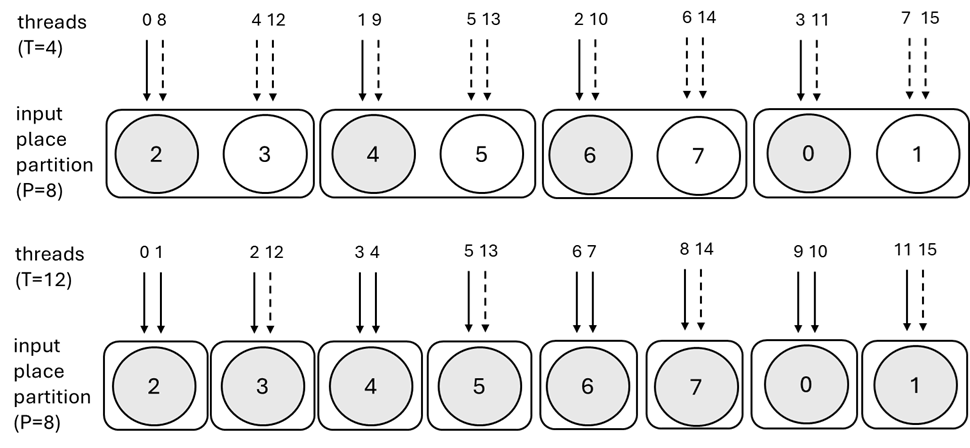
\includegraphics[width=0.7\textwidth]{figs/spread_policy}
    \caption{\kcode{spread} affinity policy}
    \label{fig:spread_policy}
\end{subfigure}

\vspace{2mm}

\begin{subfigure}[b]{0.95\textwidth}
    \centering
    \captionsetup{justification=centering}
    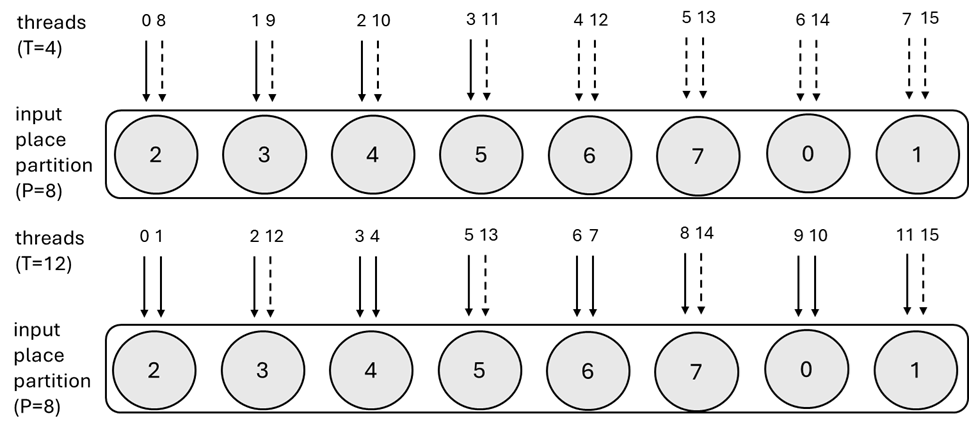
\includegraphics[width=0.7\textwidth]{figs/close_policy}
    \caption{\kcode{close} affinity policy}
    \label{fig:close_policy}
\end{subfigure}

\vspace{2mm}

\begin{subfigure}[b]{0.95\textwidth}
    \centering
    \captionsetup{justification=centering}
    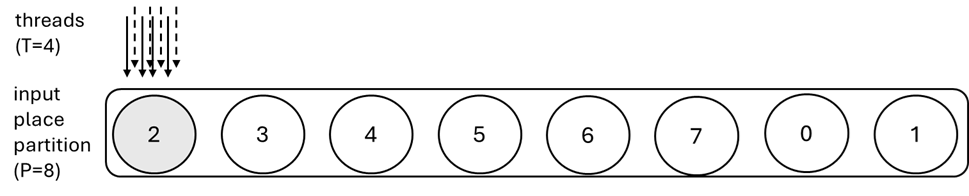
\includegraphics[width=0.7\textwidth]{figs/primary_policy}
    \caption{\kcode{primary} affinity policy}
    \label{fig:primary_policy}
\end{subfigure}

\caption{Thread Affinity Illustrations}
    \label{fig:affinity_illustrations}
\end{figure}


There are three policies:

\begin{itemize}
\item The \kcode{spread} policy divides the input place partition into
subpartitions and then distributes the threads to a place in each of the
subpartitions while setting the \plc{place-group-var} ICV for each
thread to a place group that encloses the subpartition to which it is
distributed. This policy can be useful for reducing resource
contention between threads that execute in the parallel region
or if threads are expected to spawn nested parallelism that is
confined to their new place subpartition. 

\item The \kcode{close} policy round-robin assigns threads (one or more at a
time) to places in the input place partition. The \plc{place-group-var}
ICV for each thread is set to the input place group of the region.

\item The \kcode{primary} policy is used to ensure all threads are assigned to
the same place, which is the place of the encountering thread if it is bound to
a place. Again, each thread inherits the input place group for its
\plc{place-group-var} ICV.
\end{itemize} 

Let $T$ be the team size, let $P$ be the number of places in the input place
partition, and let $G$ be the number of children (immediately nested places or
place groups) of the input place group.

For the \kcode{spread} policy, when $T < G$ each thread is assigned to one of
$T$ sets of $\lceil G/T \rceil$ or $\lfloor G/T \rfloor$ children, and
otherwise each set of $\lceil T/G \rceil$ or $\lfloor T/G \rfloor$ consecutive
threads are assigned to a different child. If the child is itself a place
group, its assigned threads are then similarly spread over its children, and
this process continues recursively. The first place of each of the
subpartitions is \emph{team-eligible} for place assignment (meaning one of the
$T$ team threads can be assigned to it).

For the \kcode{close} policy, each place in the input place partition is
team-eligible for place assignment.  Finally, for the \kcode{primary} policy
only the place to which the primary thread is assigned (or will be assigned as
chosen by the implementation) is team-eligible for place assignment.

In Figure~\ref{fig:affinity_illustrations}, the team-eligible places are depicted
as gray circles.

Let $Q$ be the number of team-eligible places in the input place partition. When
$T > Q$, the $T$ threads that comprise the team are divided into $Q$ sets of
$\lceil T/Q \rceil$ or $\lfloor T/Q \rfloor$ consecutive threads, and otherwise
they are divided into $T$ sets of one thread each. The first thread set is
assigned to the place of the primary thread if that thread is already assigned,
and otherwise the thread set is assigned to one of the $Q$ team-eligible
places. The next thread set is then assigned to the next team-eligible place,
and so on with wrap-around.

For the \kcode{spread} policy when $T > P$ or for the \kcode{close} policy,
after the $T$ threads are assigned there will be $K = P - T \bmod P$
team-eligible places with one less thread than the rest. If $K < P$, each of
the first $K$ free-agent threads that begin execution in the parallel region
will be assigned to one of these places not reserved for structured threads, in
some order defined by the implementation. The bottom case of
Figure~\ref{fig:spread_policy} and both cases of Figure~\ref{fig:close_policy}
provide an illustration of such assignments.

Any additional free-agent threads for the \kcode{spread} policy are fairly
distributed over subpartitions and their places, avoiding subpartitions or
places reserved for structured threads. See the top case of
Figure~\ref{fig:spread_policy} for an example illustration of such assignments.
For other policies, additional free-agent threads are fairly distributed over
team-eligible places, again avoiding places reserved for structured threads. 

The following example demonstrates how to control thread affinity for a
parallel region according to an affinity policy. The machine architecture
assumed for this example is depicted in Figure~\ref{fig:mach_arch}. It consists
of two sockets, each equipped with a quad-core processor and configured to
execute two hardware threads simultaneously on each core. These examples assume
a contiguous core numbering starting from $0$, such that the hardware threads
$0$,$1$ form the first physical core.

\ifpdf
\begin{figure}[htb]
\centerline{\includegraphics[width=3.0in,keepaspectratio=true]%
{figs/proc_bind_fig.pdf}}
\caption{A machine architecture with two quad-core processors}
\label{fig:mach_arch}
\end{figure}
\fi

The following equivalent place list declarations consist of eight places (which 
we designate as p0 to p7):
\begin{boxeducode}
\kcode{OMP_PLACES}="{0,1},{2,3},{4,5},{6,7},{8,9},{10,11},{12,13},{14,15}"
\end{boxeducode}
or
\begin{boxeducode}
\kcode{OMP_PLACES}="{0:2}:8:2"
\end{boxeducode}
or
\begin{boxeducode}
\kcode{OMP_PLACES}="cores"
\end{boxeducode}

\cexample[6.0]{affinity_control}{1}
%\clearpage

\ffreeexample[6.0]{affinity_control}{1}

The example is simple: a \kcode{parallel} construct in which there is a call to
an external procedure \ucode{work}. By setting \kcode{OMP_NUM_THREADS} to \pout{4}
and \kcode{OMP_THREAD_LIMIT} to \pout{16}, the construct will spawn a team of size 4
and will allow for up to 12 additional free-agent threads to join in the execution
of tasks in \ucode{work}. Note that the OpenMP 6.0 specification also allows for
\kcode{OMP_NUM_THREADS} and \kcode{OMP_THREAD_LIMIT} to be set to a
\emph{numeric abstract name}. For example, setting \kcode{OMP_THREAD_LIMIT} to
\pout{"n_threads"} will set it to the number of hardware threads available on
the device, which again is 16 for the machine we are assuming.

The thread affinity policy can then be controlled via the \kcode{OMP_PROC_BIND}
environment variable. 
If \kcode{OMP_PROC_BIND} is set to
a comma-separated list of \kcode{spread}, \kcode{close}, or \kcode{primary},
then each element of the list is used for each level of parallelism from left
to right. For example, setting \kcode{OMP_PROC_BIND} to \pout{"spread,close"}
will apply the \kcode{spread} affinity policy to the outer active
\kcode{parallel} region and a \kcode{close} affinity policy (operating within
an updated place partition) for an inner active \kcode{parallel} region.

\index{affinity!proc_bind clause@\kcode{proc_bind} clause}
\index{clauses!proc_bind@\kcode{proc_bind}}
\index{proc_bind clause@\kcode{proc_bind} clause}

The following examples demonstrate how to use the \kcode{proc_bind} clause to
control the thread binding for a team of threads in a \kcode{parallel} region.
The same machine architecture and place list from the preceding section is
assumed.

\subsection{Spread Affinity Policy} \label{subsec:affinity_spread}
\index{affinity!spread policy@\kcode{spread} policy} \index{spread
policy@\kcode{spread} policy}


The following example shows the result of the \kcode{spread} affinity policy on
the partition list when the number of threads is less than or equal to the
number of places in the parent's place partition, for the machine architecture
depicted above. Note that the threads are bound to the first place of each
subpartition.

\cexample[4.0]{affinity}{1}

\fexample[4.0]{affinity}{1}

It is unspecified on which place the primary thread is initially started. If the 
primary thread is initially started on p0, the following placement of threads will 
be applied in the parallel region:

\begin{compactitem}
\item thread 0 executes on p0 with the place partition p0,p1

\item thread 1 executes on p2 with the place partition p2,p3

\item thread 2 executes on p4 with the place partition p4,p5

\item thread 3 executes on p6 with the place partition p6,p7
\end{compactitem}


If the primary thread would initially be started on p2, the placement of threads 
and distribution of the place partition would be as follows:

\begin{compactitem}
\item thread 0 executes on p2 with the place partition p2,p3

\item thread 1 executes on p4 with the place partition p4,p5

\item thread 2 executes on p6 with the place partition p6,p7

\item thread 3 executes on p0 with the place partition p0,p1
\end{compactitem}

The following example illustrates the \kcode{spread} thread affinity policy when 
the number of threads is greater than the number of places in the parent's place 
partition.

Let \ucode{T} be the number of threads in the team, and \ucode{P} be the number of places in the 
parent's place partition. The first \ucode{T/P} threads of the team (including the primary
thread) execute on the parent's place. The next \ucode{T/P} threads execute on the next 
place in the place partition, and so on, with wrap around. 

\cexample[4.0]{affinity}{2}

\ffreeexample[4.0]{affinity}{2}

It is unspecified on which place the primary thread is initially started. If the 
primary thread is initially started on p0, the following placement of threads will 
be applied in the parallel region:

\begin{compactitem}
\item threads 0,1 execute on p0 with the place partition p0

\item threads 2,3 execute on p1 with the place partition p1

\item threads 4,5 execute on p2 with the place partition p2

\item threads 6,7 execute on p3 with the place partition p3

\item threads 8,9 execute on p4 with the place partition p4

\item threads 10,11 execute on p5 with the place partition p5

\item threads 12,13 execute on p6 with the place partition p6

\item threads 14,15 execute on p7 with the place partition p7
\end{compactitem}

If the primary thread would initially be started on p2, the placement of threads 
and distribution of the place partition would be as follows:

\begin{compactitem}
\item threads 0,1 execute on p2 with the place partition p2

\item threads 2,3 execute on p3 with the place partition p3

\item threads 4,5 execute on p4 with the place partition p4

\item threads 6,7 execute on p5 with the place partition p5

\item threads 8,9 execute on p6 with the place partition p6

\item threads 10,11 execute on p7 with the place partition p7

\item threads 12,13 execute on p0 with the place partition p0

\item threads 14,15 execute on p1 with the place partition p1
\end{compactitem}

\subsection{Close Affinity Policy}
\label{subsec:affinity_close}
\index{affinity!close policy@\kcode{close} policy}
\index{close policy@\kcode{close} policy}

The following example shows the result of the \kcode{close} affinity policy on 
the partition list when the number of threads is less than or equal to the number 
of places in the parent's place partition, for the machine architecture depicted above. 
The place partition is not changed by the \kcode{close} policy.

\cexample[4.0]{affinity}{3}

\fexample[4.0]{affinity}{3}
\clearpage

It is unspecified on which place the primary thread is initially started. If the 
primary thread is initially started on p0, the following placement of threads will 
be applied in the \kcode{parallel} region:

\begin{compactitem}
\item thread 0 executes on p0 with the place partition p0-p7

\item thread 1 executes on p1 with the place partition p0-p7

\item thread 2 executes on p2 with the place partition p0-p7

\item thread 3 executes on p3 with the place partition p0-p7
\end{compactitem}

If the primary thread would initially be started on p2, the placement of threads 
and distribution of the place partition would be as follows:

\begin{compactitem}
\item thread 0 executes on p2 with the place partition p0-p7

\item thread 1 executes on p3 with the place partition p0-p7

\item thread 2 executes on p4 with the place partition p0-p7

\item thread 3 executes on p5 with the place partition p0-p7
\end{compactitem}

The following example illustrates the \kcode{close} thread affinity policy when 
the number of threads is greater than the number of places in the parent's place 
partition.

Let \ucode{T} be the number of threads in the team, and \ucode{P} be the number of places in the 
parent's place partition. The first \ucode{T/P} threads of the team (including the primary
thread) execute on the parent's place. The next \ucode{T/P} threads execute on the next 
place in the place partition, and so on, with wrap around. The place partition 
is not changed by the \kcode{close} policy.

\cexample[4.0]{affinity}{4}

\ffreeexample[4.0]{affinity}{4}
\clearpage

It is unspecified on which place the primary thread is initially started. If the 
primary thread is initially running on p0, the following placement of threads will 
be applied in the parallel region:

\begin{compactitem}
\item threads 0,1 execute on p0 with the place partition p0-p7

\item threads 2,3 execute on p1 with the place partition p0-p7

\item threads 4,5 execute on p2 with the place partition p0-p7

\item threads 6,7 execute on p3 with the place partition p0-p7

\item threads 8,9 execute on p4 with the place partition p0-p7

\item threads 10,11 execute on p5 with the place partition p0-p7

\item threads 12,13 execute on p6 with the place partition p0-p7

\item threads 14,15 execute on p7 with the place partition p0-p7
\end{compactitem}

If the primary thread would initially be started on p2, the placement of threads 
and distribution of the place partition would be as follows:

\begin{compactitem}
\item threads 0,1 execute on p2 with the place partition p0-p7

\item threads 2,3 execute on p3 with the place partition p0-p7

\item threads 4,5 execute on p4 with the place partition p0-p7

\item threads 6,7 execute on p5 with the place partition p0-p7

\item threads 8,9 execute on p6 with the place partition p0-p7

\item threads 10,11 execute on p7 with the place partition p0-p7

\item threads 12,13 execute on p0 with the place partition p0-p7

\item threads 14,15 execute on p1 with the place partition p0-p7
\end{compactitem}

\subsection{Primary Affinity Policy}
\label{subsec:affinity_primary}
\index{affinity!primary policy@\kcode{primary} policy}
\index{primary policy@\kcode{primary} policy}

The following example shows the result of the \kcode{primary} affinity policy on 
the partition list for the machine architecture depicted above. The place partition 
is not changed by the primary policy.

\cexample[5.1]{affinity}{5}

\fexample[5.1]{affinity}{5}

It is unspecified on which place the primary thread is initially started. If the 
primary thread is initially running on p0, the following placement of threads will 
be applied in the parallel region:

\begin{compactitem}
\item threads 0-3 execute on p0 with the place partition p0-p7
\end{compactitem}

If the primary thread would initially be started on p2, the placement of threads 
and distribution of the place partition would be as follows:

\begin{compactitem}
\item threads 0-3 execute on p2 with the place partition p0-p7
\end{compactitem}



\section{Task Affinity}
\label{sec: task_affinity}
\index{affinity!task affinity}
\index{affinity!affinity clause@\kcode{affinity} clause}
\index{clauses!affinity@\kcode{affinity}}
\index{affinity clause@\kcode{affinity} clause}

The next example illustrates the use of the \kcode{affinity}
clause with a \kcode{task} construct.
The variables in the \kcode{affinity} clause provide a
hint to the runtime that the task should execute
``close'' to the physical storage location of the variables. For example,
on a two-socket platform with a local memory component
close to each processor socket, the runtime will attempt to
schedule the task execution on the socket where the storage is located.

Because the C/C++ code employs a pointer, an array section is used in
the \kcode{affinity} clause.
Fortran code can use an array reference to specify the storage, as
shown here.

Note, in the second task of the C/C++ code the \ucode{B} pointer is declared
shared.  Otherwise, by default, it would be firstprivate since it is a local
variable, and would probably be saved for the second task before being assigned
a storage address by the first task.  Also, one might think it reasonable to use
the \kcode{affinity} clause \kcode{affinity(\ucode{B[:N]})} on the second \kcode{task} construct.
However, the storage behind \ucode{B} is created in the first task, and the 
array section reference may not be valid when the second task is generated.
The use of the \ucode{A} array is sufficient for this case, because one
would expect the storage for \ucode{A} and \ucode{B} to be physically ``close''
(as provided by the hint in the first task).

\cexample[5.0]{affinity}{6}

\ffreeexample[5.0]{affinity}{6}


\section{Affinity Display}
\label{sec:affinity_display}
\index{affinity display!OMP_DISPLAY_AFFINITY@\kcode{OMP_DISPLAY_AFFINITY}}
\index{environment variables!OMP_DISPLAY_AFFINITY@\kcode{OMP_DISPLAY_AFFINITY}}
\index{OMP_DISPLAY_AFFINITY@\kcode{OMP_DISPLAY_AFFINITY}}
\index{affinity display!OMP_AFFINITY_FORMAT@\kcode{OMP_AFFINITY_FORMAT}}
\index{environment variables!OMP_AFFINITY_FORMAT@\kcode{OMP_AFFINITY_FORMAT}}
\index{OMP_AFFINITY_FORMAT@\kcode{OMP_AFFINITY_FORMAT}}
\index{affinity display!omp_display_affinity routine@\kcode{omp_display_affinity} routine}
\index{routines!omp_display_affinity@\kcode{omp_display_affinity}}
\index{omp_display_affinity routine@\kcode{omp_display_affinity} routine}

The following examples illustrate ways to display thread affinity.
Automatic display of affinity can be invoked by setting
the \kcode{OMP_DISPLAY_AFFINITY} environment variable to \vcode{TRUE}.  
The format of the output can be customized by setting the 
\kcode{OMP_AFFINITY_FORMAT} environment variable to an appropriate string.  
Also, there are API calls for the user to display thread affinity 
at selected locations within code.

For the first example the environment variable \kcode{OMP_DISPLAY_AFFINITY} has been
set to \vcode{TRUE}, and execution occurs on an 8-core system with \kcode{OMP_NUM_THREADS} set to 8.

The affinity for the primary thread is reported through a call to the API
\kcode{omp_display_affinity()} routine. For default affinity settings
the report shows that the primary thread can execute on any of the cores. 
In the following parallel region the affinity for each of the team threads is reported
automatically since the \kcode{OMP_DISPLAY_AFFINITY} environment variable has been set
to \vcode{TRUE}.

These two reports are often useful (as in hybrid codes using both MPI and OpenMP) 
to observe the affinity (for an MPI task) before the parallel region,
and during an OpenMP parallel region. Note: the next parallel region uses the 
same number of threads as in the previous parallel region and affinities are 
not changed, so affinity is NOT reported.

In the last parallel region, the thread affinities are reported
because the thread affinity has changed.

\cexample[5.0]{affinity_display}{1}[1]

\ffreeexample[5.0]{affinity_display}{1}[1]


In the following example 2 threads are forked, and each executes on a socket. Next,
a nested parallel region runs half of the available threads on each socket.

These OpenMP environment variables have been set:

\begin{boxeducode}
\kcode{OMP_PROC_BIND}="TRUE"
\kcode{OMP_NUM_THREADS}="2,4"
\kcode{OMP_PLACES}="{0,2,4,6},{1,3,5,7}"
\kcode{OMP_AFFINITY_FORMAT}="nest_level= %L, parent_thrd_num= %a, \
thrd_num= %n, thrd_affinity= %A"
\end{boxeducode}

where the numbers correspond to core ids for the system. Note, \kcode{OMP_DISPLAY_AFFINITY} is not
set and is \vcode{FALSE} by default.  This example shows how to use API routines to
perform affinity display operations.

\index{environment variables!OMP_PLACES@\kcode{OMP_PLACES}}
\index{OMP_PLACES@\kcode{OMP_PLACES}}
For each of the two first-level threads the \kcode{OMP_PLACES} variable specifies
a place with all the core-ids of the socket (\{0,2,4,6\} for one thread and \{1,3,5,7\} for the other).
(As is sometimes the case in 2-socket systems, one socket may consist
of the even id numbers, while the other may have the odd id numbers.)  The affinities
are printed according to the \kcode{OMP_AFFINITY_FORMAT} format: providing
the parallel nesting level (\ucode{\%L}), the ancestor thread number (\ucode{\%a}), the thread number (\ucode{\%n})
and the thread affinity (\ucode{\%A}). In the nested parallel region within the \ucode{socket_work} routine
the affinities for the threads on each socket are printed according to this format.

\cexample[5.0]{affinity_display}{2}[3]

\ffreeexample[5.0]{affinity_display}{2}[3]

%\newpage
\index{affinity display!omp_get_affinity_format routine@\kcode{omp_get_affinity_format} routine}
\index{routines!omp_get_affinity_format@\kcode{omp_get_affinity_format}}
\index{omp_get_affinity_format routine@\kcode{omp_get_affinity_format} routine}
\index{affinity display!omp_set_affinity_format routine@\kcode{omp_set_affinity_format} routine}
\index{routines!omp_set_affinity_format@\kcode{omp_set_affinity_format}}
\index{omp_set_affinity_format routine@\kcode{omp_set_affinity_format} routine}
The next example illustrates more details about affinity formatting.
First, the \kcode{omp_get_affinity_format()} API routine is used to 
obtain the default format. The code checks to make sure the storage 
provides enough space to hold the format.  
Next, the \kcode{omp_set_affinity_format()} API routine sets a user-defined 
format: \ucode{host=\%20H~thrd_num=\%0.4n~binds_to=\%A}.   

The host, thread number and affinity fields are specified by \ucode{\%20H}, 
\ucode{\%0.4n} and \ucode{\%A}: \ucode{H}, \ucode{n} and \ucode{A} are single character ``short names''
for the host, thread\_num and thread\_affinity data to be printed,
with format sizes of \ucode{20}, \ucode{4}, and ``size as needed''.
The period (.) indicates that the field is displayed right-justified (default is left-justified) 
and the ``0'' indicates that any unused space is to be prefixed with zeros
(e.g. instead of ``1'', ``0001'' is displayed for the field size of 4).

\index{affinity display!omp_capture_affinity routine@\kcode{omp_capture_affinity} routine}
\index{routines!omp_capture_affinity@\kcode{omp_capture_affinity}}
\index{omp_capture_affinity routine@\kcode{omp_capture_affinity} routine}
Within the parallel region the affinity for each thread is captured by 
\kcode{omp_capture_affinity()} into a buffer array with elements indexed 
by the thread number (\ucode{thrd_num}).
After the parallel region, the thread affinities are printed in thread-number order.

If the storage area in buffer is inadequate for holding the affinity
data, the stored affinity data is truncated.  
The maximum value for the number of characters (\ucode{nchars}) returned by 
\kcode{omp_capture_affinity} is captured by the \kcode{reduction(max: \ucode{max_req_store})}
clause and the \ucode{if(nchars >= max_req_store) max_req_store=nchars} statement. 
It is used to report possible truncation (if \ucode{max_req_store} > \ucode{buffer_store}).

\pagebreak
\cexample[5.0]{affinity_display}{3}

\ffreeexample[5.0]{affinity_display}{3}


%\newpage
\section{Affinity Query Functions}
\label{sec: affinity_query}
\index{affinity query!omp_get_num_places routine@\kcode{omp_get_num_places} routine}
\index{routines!omp_get_num_places@\kcode{omp_get_num_places}}
\index{omp_get_num_places routine@\kcode{omp_get_num_places} routine}
\index{affinity query!omp_get_place_num routine@\kcode{omp_get_place_num} routine}
\index{routines!omp_get_place_num@\kcode{omp_get_place_num}}
\index{omp_get_place_num routine@\kcode{omp_get_place_num} routine}
\index{affinity query!omp_get_place_num_procs routine@\kcode{omp_get_place_num_procs} routine}
\index{routines!omp_get_place_num_procs@\kcode{omp_get_place_num_procs}}
\index{omp_get_place_num_procs routine@\kcode{omp_get_place_num_procs} routine}
\index{affinity!spread policy@\kcode{spread} policy}
\index{spread policy@\kcode{spread} policy}
\index{environment variables!OMP_PLACES@\kcode{OMP_PLACES}}
\index{OMP_PLACES@\kcode{OMP_PLACES}}

In the example below a team of threads is generated on each socket of
the system, using nested parallelism. Several query functions are used
to gather information to support the creation of the teams and to obtain 
socket and thread numbers.

For proper execution of the code, the user must create a place partition, such that
each place is a listing of the core numbers for a socket. For example,
in a 2 socket system with 8 cores in each socket, and sequential numbering
in the socket for the core numbers, the \kcode{OMP_PLACES} variable would be set
to "\{0:8\},\{8:8\}", using the place syntax \{\splc{lower_bound:length:stride}\},
and the default stride of 1.

The code determines the number of sockets (\ucode{n_sockets})
using the \kcode{omp_get_num_places()} query function.
In this example each place is constructed with a list of 
each socket's core numbers, hence the number of places is equal
to the number of sockets. 

The outer parallel region forms a team of threads, and each thread 
executes on a socket (place) because the \kcode{proc_bind} clause uses 
\kcode{spread} in the outer \kcode{parallel} construct.
Next, in the \ucode{socket_init} function, an inner parallel region creates a team 
of threads equal to the number of elements (core numbers) from the place
of the parent thread. Because the outer \kcode{parallel} construct uses 
a \kcode{spread} affinity policy, each of its threads inherits a sub-partition of 
the original partition.  Hence, the \kcode{omp_get_place_num_procs} query function
returns the number of elements (here procs = cores) in the sub-partition of the thread.  
After each parent thread creates its nested parallel region on the section,
the socket number and thread number are reported.

Note: Portable tools like hwloc (Portable HardWare LOCality package), which support
many common operating systems, can be used to determine the configuration of a system.  
On some systems there are utilities, files or user guides that provide configuration
information.  For instance, the socket number and proc\_ids for a socket 
can be found in the /proc/cpuinfo text file on Linux systems.

\cexample[4.5]{affinity_query}{1}

\ffreeexample[4.5]{affinity_query}{1}



